\documentclass[12pt,a4paper]{article}
\usepackage[utf8]{inputenc}
\usepackage[left=3cm,right=2cm,top=3cm,bottom=3cm]{geometry}
\usepackage[french]{babel}
\usepackage{enumerate}
\usepackage{ulem}
\usepackage{graphicx}
\usepackage{url}
\usepackage{listings}
\usepackage{xcolor}

\begin{document}
\begin{titlepage}
\begin{center}
% Upper part of the page
\begin{center}

\includegraphics
[width=9cm]{logo.png}
\end{center}


%\textsc{\LARGE UNIVERSITE BORDEAUX 1 }\\[1.5cm]
\textsc{\huge \bfseries Memoire de projet de programmation}\\[1.5cm]
\textsc{\huge \bfseries VPN EveryWhere }\\[1.5cm]
%title

% Author and supervisor

\Large \begin{flushleft}\textbf{Par:}\\
LIU Song\\
Aissous Amin\\
HOCINI Mohamed Fouad\\
Si SABER Mohamed Amine\\
\end{flushleft}

\Large 
\begin{flushright}\textbf{Client:}\\
Samuel Thibault\\

\textbf{Chargé de TD :}\\
Henri Derycke\\
\end{flushright}


\vfill
% Bottom of the page
{\large \today}
\end{center}
\end{titlepage}
\newpage

\begin{flushleft}
\Large\textbf{Résumé }
\end{flushleft}

Dans ce projet intitulé VPN EveryWhere, notre travail était de développer un logiciel facilitant la configuration du client OpenVPN afin de simplifier l'utilisation aux différents utilisateurs quelques soit leurs niveaux en informatique, afin de pouvoir se connecter au serveur OpenVPN l'utilisateur devrait configurer le client installé sur sa machine à chaque connexion et cette tache n'est pas faisable pour le grand public.\\

Dans ce but on a rendu la configuration du client OpenVPN de FDN automatique en créant une interface, simple et facile à utiliser, il suffit juste de cliquer sur le bouton Connect et tout le travail nécessaire pour la configuration du client OpenVPN jusqu'au lancement de la connexion avec le serveur se fait automatiquement, et pour cela la bibliothèque scan qui contient les différents type de scan de ports(socket, avec et sans thread, en TCP et en UDP) récupère l'adresse du serveur à partir du fichier de configuration afin que scan des port se lance jusqu'à ce qu'il trouve un port ouvert ou non si tout les ports sont fermés, tout en commençant par le scan UDP et après on passe au scan TCP en respectant l'heuristique qu'on a mis en place en créant trois niveaux de priorité pour rendre le scan vite tout en dépendant du serveur et des ports ouverts en commençant par le niveau 1 qui contient les port les plus connus, après on passe au niveau 2 qui contient les ports qu'on a déjà trouvé ultérieurement et qui n'appartiennent pas au niveau 1 et qui se mis à jour à chaque fois où on tombe sur un port ouvert qui n'existe dans cette liste et après y a le niveau 3 qui contient tout les port possible.\\

Après avoir trouver un port ouvert le scan des port s'arrête et le fichier de configuration se mis à jour en écrivant le numéro de port ouvert trouvé et le protocole utilisé UDP ou TCP, et le client OpenVPN se lance automatiquement en prenant le fichier de configuration qui contient tout les informations nécessaire.\\



\textbf{Mots-clefs:} Vpn ,Client OpenVpn, Bibliothèque Scan tcp/udp ,  Niveaux de scan, génération de fichier de configuration.\\

\begin{flushleft}
%\Large\textbf{Abstract }
\end{flushleft}

%here abstract!!!!!\\
%\textbf{Keywords:} Vpn ,Client OpenVpn, Bibliothèque Scan tcp/udp ,  Niveaux de scan, génération de fichier de configuration.\\
\newpage

\tableofcontents 
\newpage

\textsc{\LARGE \bfseries Introduction }\\  \\ 

    Aujourd’hui, près de 2,5 milliards de personnes utilisent Internet pour communiquer et fournir/obtenir des informations.
Lorsque la communication concerne des informations sensibles telles que des coordonnées bancaires,des numéros de cartes de crédit, des dossiers médicaux, etc..., la méthode de communication doit être sécurisée.
L’échange d’informations sur internet n’est pas sécurisé par défaut, ce qui induit un risque variable d’attaques malveillantes telles que la corruption des données, l’usurpation d’identité, etc... et pour cela on utilise les VPN, alors c'est quoi un VPN ? \\

    Un réseau privé virtuel VPN (de l'anglais Virtual Private Network ) est une technologie qui crée une connexion sécurisée et cryptée entre un internaute et les sites internet qu'il visite. Ce système est utilisé depuis de longues années par les grandes entreprises, les établissements d'enseignement supérieurs et les organismes gouvernementaux qui considère la sécurité et la confidentialité de leurs communications comme une préoccupation majeure.
\\

     Alors Le rôle d'un VPN (Virtual Private Network) est de fournir aux utilisateurs et administrateurs du système d'information des conditions d'exploitation, d'utilisation et de sécurité à travers un réseau public identiques à celles disponibles sur un réseau privé. Et aussi permet originellement à un utilisateur nomade de se connecter à un réseau d'entreprise depuis l'autre bout du monde: son ordinateur portable a alors l'impression d'être directement branché au réseau d'entreprise, les paquets passant en fait de manière chiffrée via internet.\\
	
Ces réseaux offrent des avantages majeurs: \\

\begin{itemize}
\item[-] La sécurité et la confidentialité des données: permet à l'utilisateur de crypter sa connexion.\\
\item[-] Le VPN permet de contourner la géo-censure sur Internet: La géo-censure est un système de restriction qui bloque l’accès à un contenu en ligne.\\
\item[-] Le VPN garde l'anonymat : En utilisant un VPN, ce n’est plus votre adresse IP qui est connu des sites que vous visitez, mais l’adresse IP de votre VPN. \\
\end{itemize}

Malheureusement l'utilisation et la configuration des VPN n'est pas une tache facile à réaliser par tout le monde, ce qui est l'intérêt de notre projet qui consiste à faciliter l'utilisation du VPN avec une configuration automatique pour qu'il soit destiné au grand public et pas forcément à ceux qui ont des connaissances dans le domaine.\\
\newpage

\section{Étude de l'existant}
Un VPN permet d'accéder à des réseaux distants comme si on était connecté à un réseau local, et il permet aussi de protéger les données sensibles. Donc ça sera intéressant que tout le monde puissent l'utiliser.\\

FDN (French Data Network) est un fournisseur d'accès à Internet associatif.
Créé en juin 1992, c'est le plus ancien FAI de France encore en activité. Fonctionnant de manière totalement bénévole et désintéressée, l'association fournit aujourd'hui quelques centaines de lignes ADSL et de VPN à travers le pays.\\

Depuis 2013, FDN propose à ses membres des tunnels chiffrés (dits VPN).
Usages typiques du VPN de FDN :
\begin{itemize}
\item[•]Retrouver un réseau propre (IPv4 et IPv6, fixes, routées par FDN) par dessus un accès à Internet fourni par un autre opérateur (une fibre optique prise chez un grozopérateur, par exemple). FDN devient alors votre FAI, le grozopérateur n’étant plus qu’un loueur de tuyau.\\
\item[•]Gagner en sécurité sur une connexion en laquelle vous n’avez pas confiance : tous les échanges entre votre ordinateur et FDN sont chiffrés, le trafic ne peut plus être écouté sur votre réseau local.\\
\end{itemize}

OpenVPN - Open Source VPN, qui est un client VPN,  il permet de se connecter a un serveur VPN  en lui fournissant le fichier de configuration fournit par le Serveur VPN à des pairs de s'authentifier entre eux à l'aide d'une clé privée partagée à l'avance, de certificats électroniques ou de couples de noms d'utilisateur/mot de passe. Mais sa configuration qui n'est pas facile à utiliser tout les gens qui ne sont pas de bonne notion en informatique ou dans le domaine de réseaux. et malheureusement il n'existe pas à notre connaissance un outils qui permet de facilité l'utilisation d'un VPN \\

Typiquement, dans un aéroport ou dans un réseau wifi public ou d'invité . La plupart des ports sont fermés. ce qui fait qu'il se pourrait nous pouvons pas utiliser le port indiquer dans le fichier de configuration pour se connecter  serveur VPN typiquement c'est le port 1194, d'ou appariait l'utilité de scanner les ports ouvert qui sont autoriser par le fournisseur d'accès l'interner.\\

Parmi les outils de scan de port y a la bibliothèque Nmap(“Network Mapper”) est un outil open source d'exploration réseau et d'audit de sécurité. En général Nmap utilise pour les audits de sécurité mais de nombreux gestionnaires des systèmes et de réseau l'apprécient pour des tâches de routine comme les inventaires de réseau, la gestion des mises à jour planifiées ou la surveillance des hôtes et des services actifs.\\

Nous avons essayé d'utiliser la bibliothèque Nmap dans notre projet pour le scan ds ports en UDP/TCP, nous avons vite abandonner l'idée par ce que le résultat donnés par le scan udp de Nmap n'etait pas satisfaisant ca ne permettait pas de déterminer si un port et ouvert ou filtré en UDP.\\

Nous avons lancé notre projet \textbf{$<<VPEVERYTHERE>>$}, pour faciliter la configuration du serveur openvpn, et pour résoudre le problème où le cas où le port indiquer dans le fichier de configuration fournit par le serveur VPN qui ne fonctionne pas. en fin que les utilisateurs qui connaissent pas du tout le domaine, ils peuvent utiliser le VPN sans aucun difficulté.
\newpage

\section{Analyse des besoins}

Le projet a pour but d'arriver à se connecter à un serveur VPN (OpenVPN de FDN dans notre cas) avec une simple manipulation qui va lancer la configuration automatique du client en passant par le scan des ports, la génération du fichier de configuration et le lancement avec le serveur.
\subsection{Diagramme}
Voici le diagramme qui montre le fonctionnement et le déroulement des différentes taches:\\

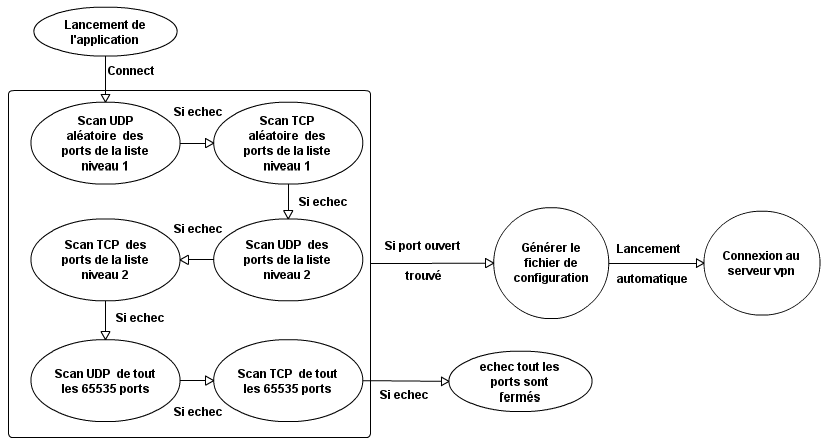
\includegraphics
[width=15cm]{FonctionnementProjet.png}
\begin{center}
{\textbf{FIGURE 01:} Fonctionnement du projet}
\end{center}

Le diagramme du fonctionnement de projet ci dessus dans la \textbf{Figure 01}, montre les différentes taches commençant par l'appel de la bibliothèque qui contient les différents types de scan (UDP, TCP avec et sans thread), et le reste des taches dépend des résultats du scan, si on trouve pas un port ouvert on marque un échec de connexion sinon on passe au génération du fichier de configuration et le lancement avec le serveur.\\

Par ailleurs, les cas d’utilisations sont décrits par le UseCase suivant: (cf. Figure 02)
\begin{center}
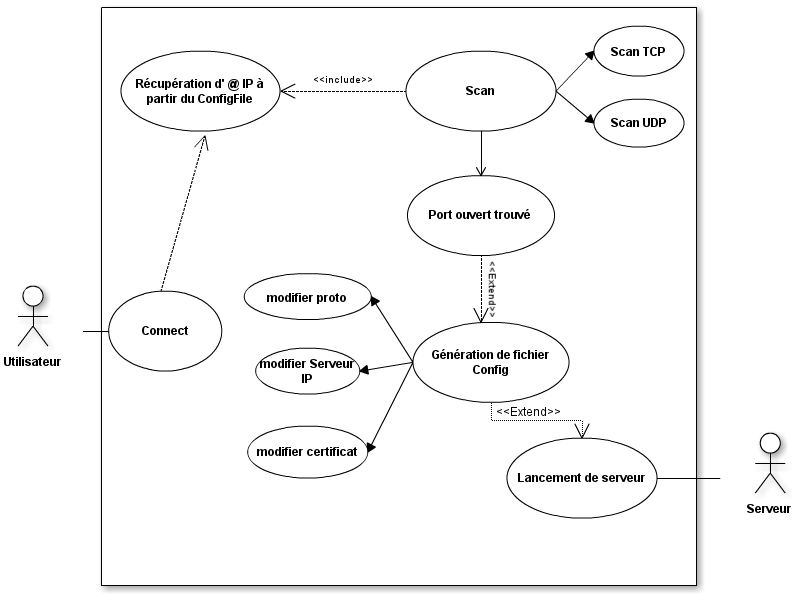
\includegraphics
[width=12cm]{Use_Case.png}\\
{\textbf{FIGURE 02:} UseCase}
\end{center}

Le diagramme de cas d'utilisation ci dessus donne une vision globale du comportement de notre application, on a deux acteurs: l'utilisateur et le serveur.\\

L'utilisateur : celui qui utilise notre logiciel, lorsqu'il clique sur connect, cette action vas lancer la connexion avec le serveur en passant par plusieurs action : Récupération d'adresse du serveur a partir du fichier de configuration, lacement du scan et la génération du fichier de configuration.\\

Serveur : c'est le serveur OpenVpn distant qu'on essaye a se connecté avec.\\
\subsection{Besoins fonctionnels}

Notre projet se résume dans la configuration automatique du VPN, il est organisé par priorité sur quatre phases essentiels, qui se résume comme suit:

\paragraph{ Le scan des ports: }c'est la phase la plus importante de notre travail, elle consiste à rechercher les ports qui permettraient de se connecter au serveur VPN, au début on sait pas quels ports sont ouverts lesquels sont fermés et c'est impossible de scanner tout les ports à la fois, parce que la carte réseaux ne supportera pas autant de connexions et aussi ça risque que le fournisseur du réseau nous bloque et nous mettre dans sa blacklist, on a mis en place une heuristique en passant par trois niveaux de scan pour éviter de tomber sur ce cas et aussi pour améliorer la recherche des ports.\\

Dans la figure ci dessous, on voit que pour se connecter au serveur, y a trois types de ports: soit le port est ouvert et c'est le serveur qui répond, soit le port est ouvert mais y a un proxy transparent qui répond et non pas le serveur, soit le port est fermé.\\
\begin{center}
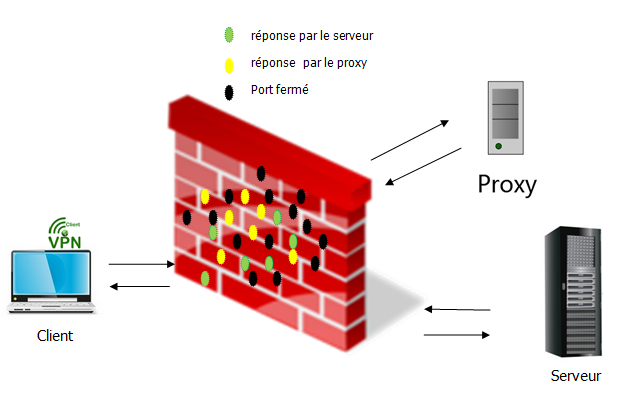
\includegraphics
[width=10cm]{Scan.png}\\
{\textbf{FIGURE 03:} Scan }
\end{center}

La figure ci dessous montre le diagramme du besoin fonctionnel scan:

\begin{center}
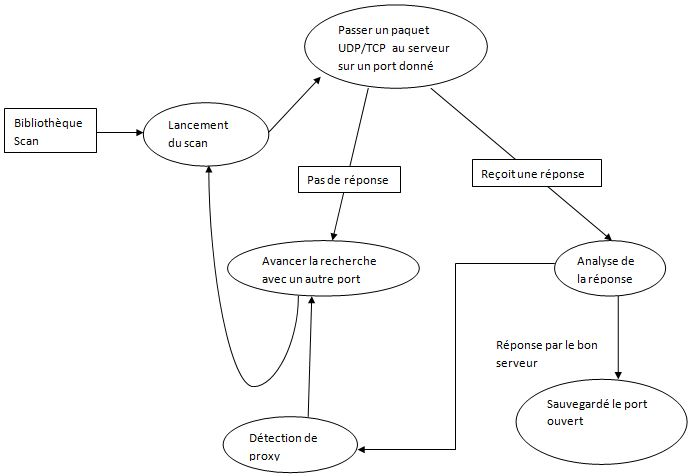
\includegraphics
[width=14cm]{Graphedesbesoinsfonctionnels0.JPG}
{\textbf{FIGURE 04:} Graphe des besoins fonctionnels }
\end{center}

Le diagramme montre les deux possibilités du scan, soit on trouve pas le port ouvert, et dans ce cas la on avance le scan avec un autre port, soit on trouve le port ouvert,dans ce cas on analyse le paquet reçu pour différencier entre un proxy transparent et le serveur OpenVpn, si la réponse vient du proxy on continu le scan avec un autre port.

\paragraph{Génération du fichier de configuration: }une fois que la phase scan des ports qui permettons de trouver un port ouvert est fini, en utilisant le  numéro de port trouvé, le protocole utilisé UDP ou TCP dans la phase précédente et le fichier de configuration.ovpn fourni par le Serveur OpenVPN  on adapte ce dernier qui contiendra les informations nécessaire à la connexion au Serveur(Numéro de port, protocole, user, password, adresse du serveur, certificat...) avec les données précédentes.

\paragraph{Lancement avec le serveur: }consiste à lancer la connexion automatique du client avec le serveur en utilisant la configuration précédente.

\paragraph{Test: } 
Pour la partie test, on a utilisé plusieurs approche afin d'être sur des résultats obtenus tel que la comparaison des résultats de notre scan avec des bibliothèques qui existe déjà comme nmap qu'on a utilisé au début...etc, et on va parler de ça en détails dans ce qui suit.

\subsection{GUI et Graphe de Fonctionnement de l'interface}
\textbf
Notre application va permettre à un client de se connecter facilement à un serveur VPN, on a décidé après plusieurs rencontres avec le client de faire une interface simple et pratique tout on ajoutant des fonctionnalités avancées pour les utilisateurs expérimentés, la figure ci dessous montre les différentes fonctionnalités de notre interface. \\
\begin{center}
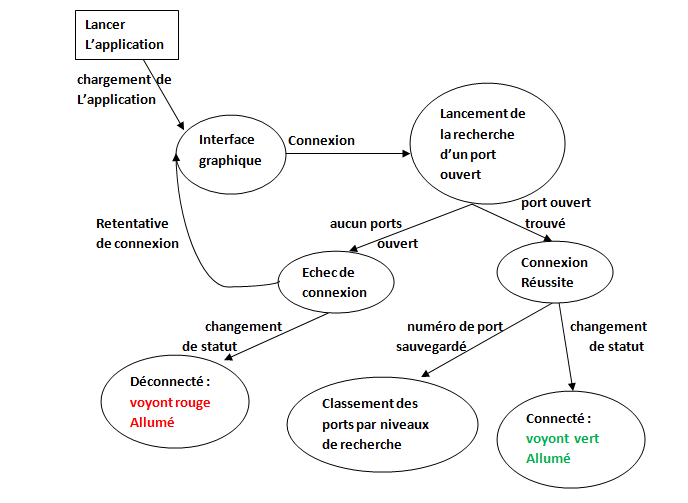
\includegraphics
[width=13cm]{Graphedefonctionement.png}\\
{\textbf{FIGURE 05:} Graphe de Fonctionnement de l'interface}
\end{center}



\subsection{Besoins non fonctionnels}
\subsubsection{Besoins comportementaux}

\paragraph{2.4.1.1 Vitesse: }
La bibliothèque doit être capable de faire un scan des ports dans un temps raisonnable en quelques dizaines de seconds, sauf dans le cas de la recherche exhaustive ou cela pourra prendre un peu plus de temps.
\paragraph{2.4.1.2 Facilité d'utilisation: }
Notre application est destiner au large publique la facilité d’utilisation est primordial, chaque utilisateur quel que soit son niveau de connaissance en informatique doit être capable de l’utiliser c’est pour cela qu’on a opter pour une interface simple d’utilisation, où le fait de cliquer simplement sur le bouton Connect lancera le scan des ports et la génération du fichier de configuration .CUBE ainsi éventuellement la connexion automatique au serveur VPN (cela dépendra de l’avancement du projet ) , si la connexion est réussi un voyant vert s’allume sinon dans le cas contraire le voyant sera rouge.\\

L'interface donne la possibilité aux utilisateurs plus expérimenté dans le domaine informatique de faire une configuration manuelle des paramètres de connexion au serveur VPN,et d'ouvrir le fichier .cube de configuration.\\
Elle doit aussi être facile à installer.
 \setlength{\parskip}{1ex}
\paragraph{2.4.1.3 Robustesse: }
S’il y a un échec dans la recherche des ports la bibliothèque doit être capable de relancer le scan, elle temporise pendant 15 seconde puis refait un nouveau scan de ports car il se pourrait que lors du scan précèdent la recherche n’avait pas donné de résultats car il y’avais un problème de connexion dans le réseau.
\paragraph{2.4.1.4 Les difficultés techniques: }
\begin{itemize}
\item[] \textbf{Réduire le temps d’attente: }
Faire un scan de tous les ports dans le cas où  les ports les plus connus ne permettent pas la connexion au Serveur VPN cela augmentera le temps de réponse la difficulté c’est de trouver un mécanisme qui permet de réduire ce temps d’attente.\\
\item[] \textbf{Quand es ce arrêter le scan des ports?: }
Vu que l’application est amenée à travailler dans n’importe quel type de réseau il se pourra qu’elle soit lancé dans un réseau dont la connexion internet n’est pas stable, cela pourra fausser le résultat du scan des ports en indiquant qu’aucun port ne permet de se connecter au VPN, La difficulté est de définir si on doit relancer le scan des ports ou dire que ce n’est pas possible de trouver des ports qui parementent la connexion au serveur VPN, nous avons opter de relancer un deuxième scan automatiquement puis on laissera le choix à l’utilisateur s’il veut réessayer ou pas.
\end{itemize}
\begin{itemize}
\item[] \textbf{Limitation de nombre des connexions ouvertes: }
Lors du scan des ports il ne faut pas essayer de tester tous les ports à la fois car chaque réseau a un nombre maximal de connexion ouvertes en parallèle, par exemple pour le réseau Free le nombre maximal de connexions parallèle autorisé est de 100.\\

\subsubsection{Besoins organisationnels}

\item[] \textbf{Processus de développement: }\\
\begin{itemize}
\item L’équipe est constituée de 4 membres, ayant des tâches qui peuvent ou non être faites en binôme.\\
\item Le projet sera réalisé avec le langage Python\\
\item Le scan des ports doit être sous forme bibliothèque python.
\end{itemize}
\end{itemize}

\subsubsection{Besoins externes}

\paragraph{2.4.3.1 Contraintes de Portabilité: }
L’application doit être utilisable sur différents système d’exploitation (Linux, Windows et MAC OS)

\paragraph{2.4.3.2 Contraintes légales:}
L’implémentation de la phase La recherche des ports sera sous forme de bibliothèque python afin qu'elle puisse être réutilisable dans d'autres projets, le code doit être bien clair avec des commentaires en anglais ceci afin de facilité sa réutilisation par d’autre personne.\\

Puisque la bibliothèque réalisant le scanne des ports sera réutilisé dans d’autres projets, nous avons choisi de la mettre l’application sous licence LGPL afin de permettre sa modification et sa distribution.\\
\subsubsection{Gestion du temps}
\textbf{Diagramme de Gantt:}
Ce diagramme représente visuellement les diverses tâches composant notre projet en fonction du temps.
\begin{flushleft}
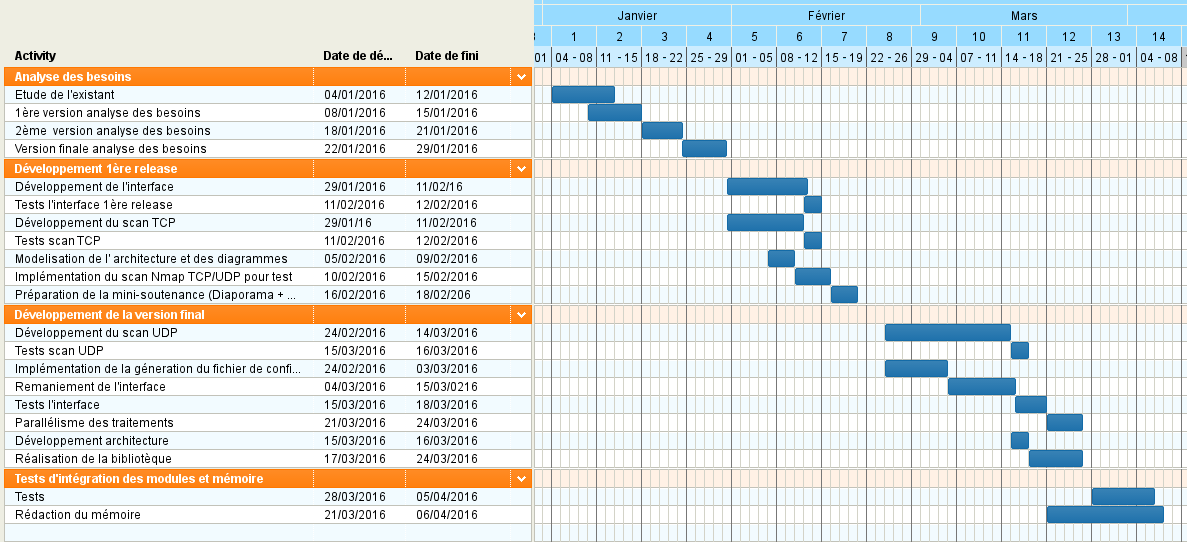
\includegraphics
[width=17cm]{DiagrammeGantt.png}

\end{flushleft}
\begin{center}
{\textbf{FIGURE 06:} Diagramme de Gantt }
\end{center}

\subsection{Diagramme de séquence }

Le diagramme de séquence si dessous présente les messages échangés entre les
différents taches.\\
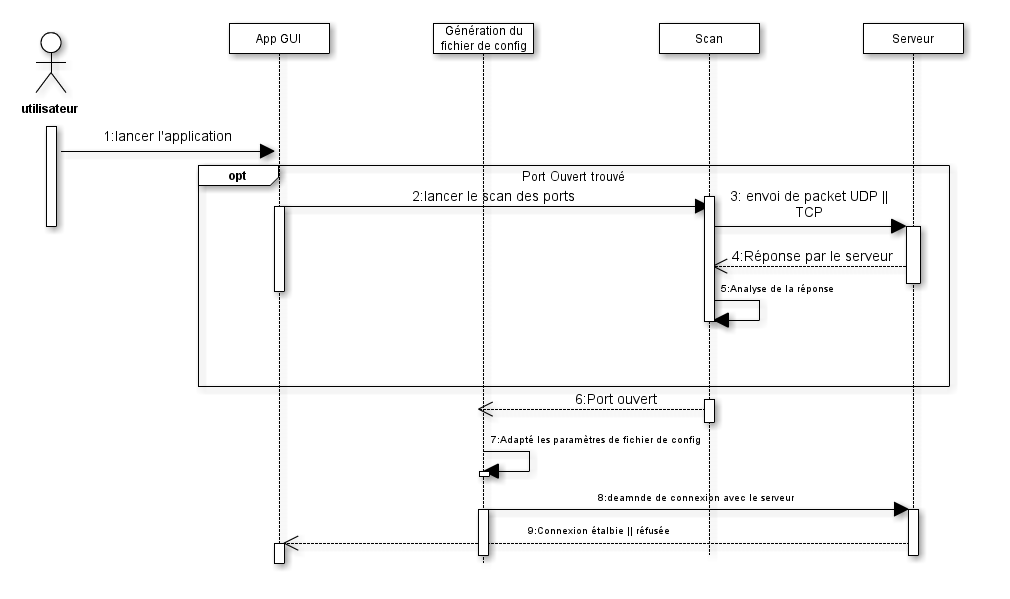
\includegraphics
[width=15cm]{Diagramme_sequence.png}
\begin{center}
{\textbf{FIGURE 07:} Diagramme de séquence de l'action connect}
\end{center}

Lorsque l'utilisateur lance l'application une interface s'affiche, le fait de cliquer sur le bouton connect lance un message d'appel de la bibliothèque scan, et cette dernière renvoi un message avec le port ouvert, vers la tache génération de fichier du configuration, afin qu'il se mis a jour, et enfin un message de demande de connexion sera envoyé vers le serveur visé.
\subsection{Type d'erreurs}
\begin{enumerate}
\item \textbf{Échec de connexion: }\\
si on trouve pas de port ouvert.\\
\item \textbf{Échec de login: }\\
si login ou password ne sont pas correct.\\
\item \textbf{Échec de certificats: }\\
si le certificats d'utilisateur est invalide ou périmé.\\
\end{enumerate}
%\subsection{Risque et parades}
\newpage


\section{Architecture}


\subsection{Vue d’ensemble}

   Mettre au point une bibliothèque python nécessite la maîtrise et l'utilisation de certain outils, essentiellement le langage python. Par conséquence, dans l'architecture de notre projet on a essayé de respecter les méthodes d'approche objet le maximum possible prenant on considération que c'est un peu difficile de faire ça dans notre cas.
   
   Voici en premier lieu un diagramme de paquetages reprenant une vue globalisée sur l'architecture de l'interface.

\begin{center}
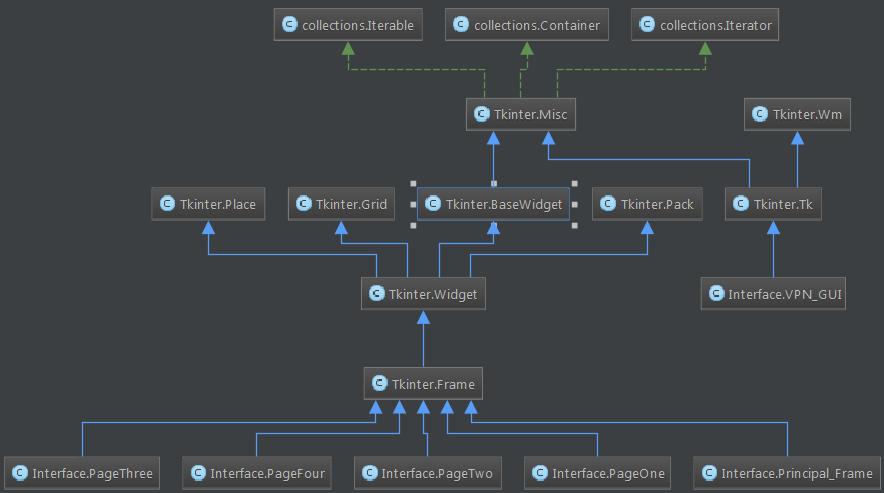
\includegraphics
[width=11cm]{pactage.png}
\end{center}
\begin{center}
{\textbf{FIGURE 08:} paquetage }
\end{center}
   
    
\subsection{Architecture de l'application (VPN EVERYWHER)}

Dans l'implémentation de notre application nous avons essayé de respecter le patern de conception 	MVC (modèle , vue , contrôleur ) qui se compose de trois fichiers python, le premier est la bibliothèque qui contient toutes les fonctionnalités de scan de port et qui sera appelée par la suite, le deuxième fichier s'occupe la génération de fichier de configuration avec toutes les informations données par l'utilisateur et par la bibliothèque, et le dernier c'est l'interface graphique qu'on a essayé de la rendre le plus simple possible.
\begin{center}
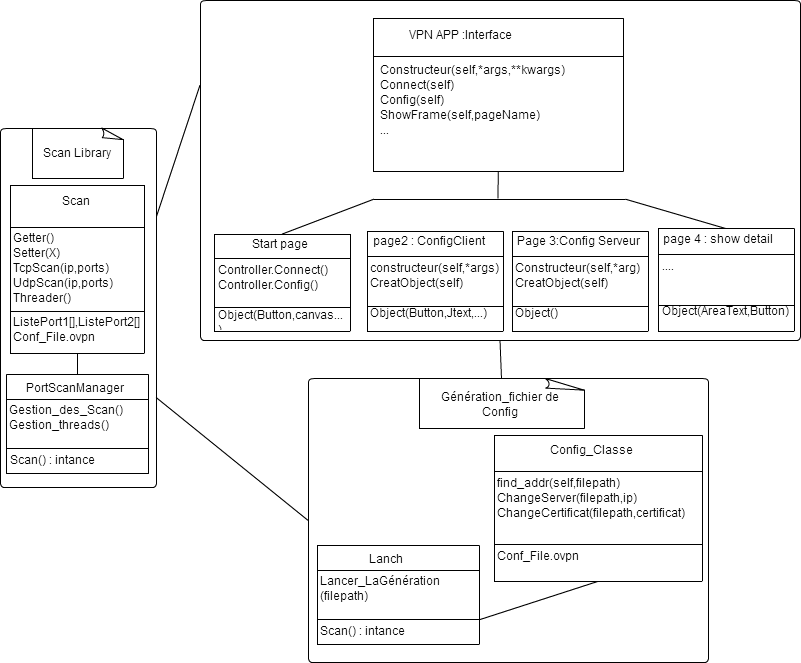
\includegraphics
[width=11cm]{Architecture.png}
\end{center}
\begin{center}
{\textbf{FIGURE 09:} Architecture }
\end{center}
\subsection{Diagrammes de classe}


Voici le diagramme de classes qui présente les différentes classes de l'application ainsi que les différentes relations entre celles-ci.
 
\begin{center}
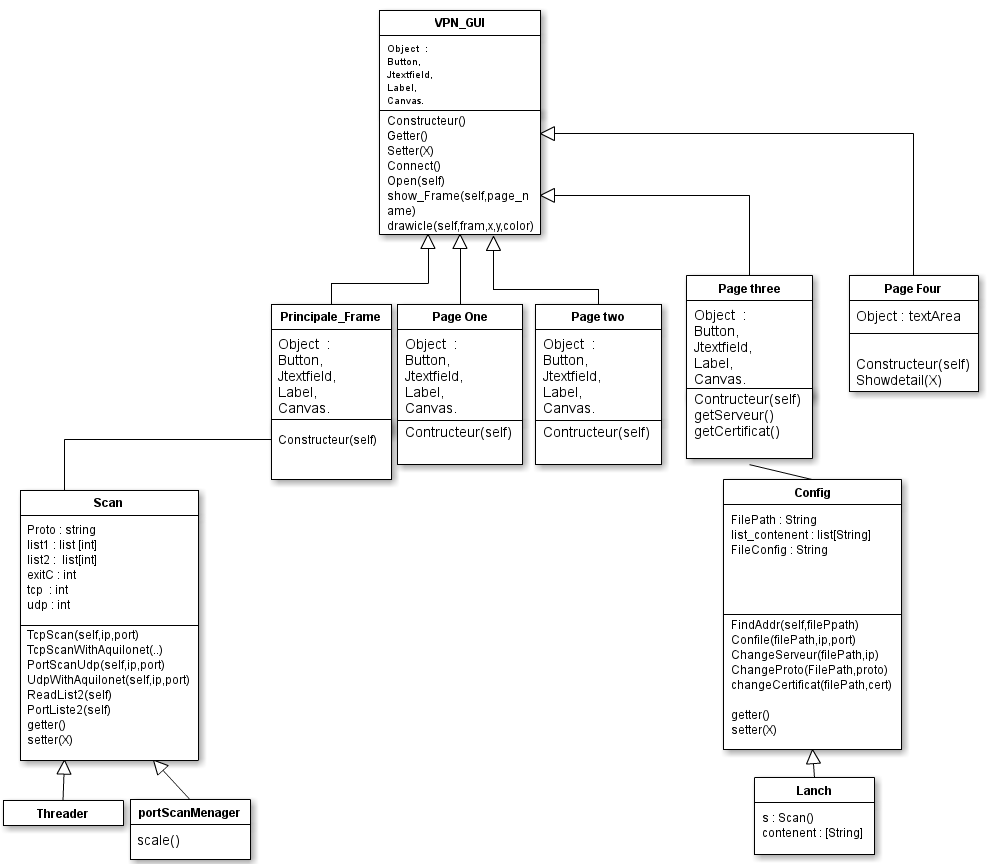
\includegraphics
[width=15cm]{Diagramme_Class.png}
{\textbf{FIGURE 10:} Diagramme de Classe }
\end{center}
%\subsection{Application de test}

On a 3 classe principale qui sont :
\begin{itemize}
\item[•] VPN GUI : Représente l'interface elle a des sous classes (pageOne...pageFour) qui représente la fenêtre principale, la fenêtre Config et la fenêtre Server.

\item[•] Scan : Représente la bibliothèque scan et elle a deux sous classes, la classe threader qui gère les threads et la classe portScanMenager qui gère les différents fonctions du scan.

\item[•] Config : contient les différents fonctions permettant la génération de fichier du configuration. la sous classe lanch permet de faire un appel de PortScanManager afin de récupéré le le bon port et lancer la génération de fichier du configuration, cette classe contient aussi tout les traitements qui permettent à mettre à jour le fichier de configuration avec les différents paramètres (Login, Password, Certificat, Protocole,  port...etc).
 
\end{itemize}
\newpage
\section{Implémentation}

L’architecture de notre projet étant désormais définie, nous allons expliquer dans ce chapitre les différentes approches utilisées dans la réalisation de chaque scan.

Le développement de notre application (VPN EVREYWHERE) c’est fait en s’utilisant le langage Python  car c’était l’une des exigences du client.
\subsection{Heuristique}

	Prenant en considération qu'on peut pas lancer un scan des 65535 ports au même temps parce que la carte réseaux ne supportera pas autant de connexions et aussi ça risque que le fournisseur du réseau nous bloque et nous mettre dans sa blacklist, pour cela on a utilisé une heuristique  pour éviter de tomber dans ces cas et avoir plus de chance de trouver un port ouvert le plus vite possible et qui consiste à faire le scan sur trois niveaux, le premier niveau contient la liste d'une dizaine de ports les plus connus et qu'on va scanner en lançant notre application, si on trouve pas de port ouvert sur le premier niveau on passe au deuxième qui contient la liste des ports qui n'appartient pas au premier niveau et qui étaient ouvert pendant les dernière connexions, si on trouve pas de port ouvert sur les deux premier niveaux on passe au troisième pour scanner aléatoirement tout les ports en lançant une dizaine à la fois.

\subsection{Bibliothèque Scan des ports (UDP/TCP)}

Pour répondre aux exigences du cahier des besoins qui demandaient de réaliser une bibliothèque de Scan de ports TCP/UDP en python qui soit réutilisable dans d’autres projets,  Nous avons réalisé 4 fonctions de scan de ports.\\
\begin{itemize}
\item[•]Les fonctions \textbf{(TcpScan ()/PortScanUdp())} sont utilisées dans un cas général où on est amené à scanner les ports en (TCP/UDP) de n’importe quel serveur VPN., c’est les fonctions qui pourraient être réutilisé dans d’autres projets. 

\item[•]Les fonctions \textbf{(TcpScanWithAquilonet ()/PortScanUdpWithAquilonet())} réalisent le scan des ports d’un cas bien particulier, elles réalisent le scanne des ports ouverts en UDP/TCP qui permettent la connexion au serveur vpn-rw.fdn.fr, ce dernier écoute sur tous les ports en UDP/TCP. Par la suite nous allons aborder cela beaucoup plus en détails.
\end{itemize}
Il est à noter que dans l’implémentation de la bibliothèque réalisant le scan des ports, nous avons privilégié l’utilisation du protocole UDP au lieu du TCP pour des raisons liées au temps de réponses des deux approches. En effet le protocole UDP est un protocole non orienté connexion ce qui fait que le temps de réponse de l’application utilisant le protocole UDP sera meilleur que celui donner par le protocole TCP, ceci dit l’utilisation du protocole UDP n’est pas toujours possible par exemple dans le cas où un port n’est ouvert qu’en TCP.

Dans ce qui suit nous allons détailler chaque type de scan implémenté et aussi expliquer les choix d’implémentation que nous avons dû faire.

\subsection{Le scan des ports TCP/UDP de n’importe quel serveur VPN (cas général):}
\subsubsection{Scan TCP(TcpScan ())}

La réalisation du scan des ports en TCP d’un serveur VPN est relativement simple, vu que le protocole TCP est un protocole orienté connexion il a suffi d’envoyer une requête de connexion TCP au serveur VPN via un port donné et attendre l’acquittement de la requête (une réponse ACK a la requête) de la part du serveur VPN, si la connexion réussi alors cella voudrai dire que le serveur a répondu par un ACK et que le port utilisé pour lancer la connexion au serveur est ouvert. 
\begin{flushleft}
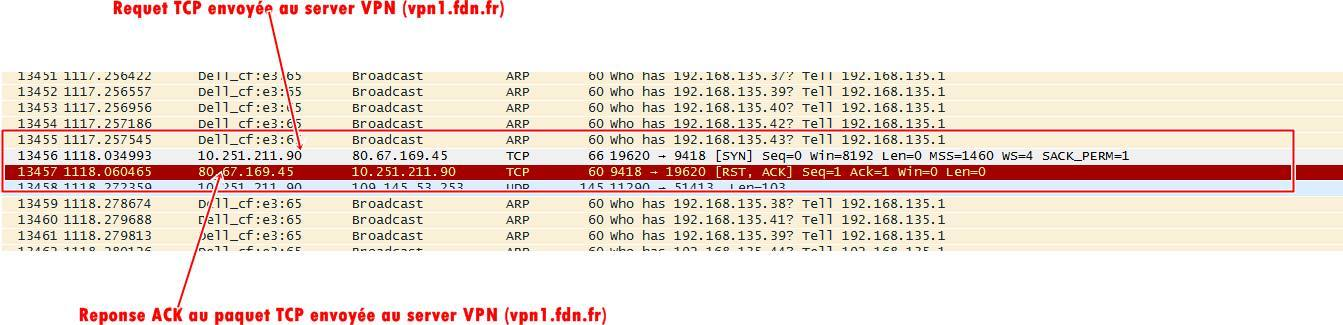
\includegraphics
[width=17cm]{ScanTcp.jpg}
\end{flushleft}
\begin{center}
{\textbf{FIGURE 11:} SCAN TCP}
\end{center}
%\subsubsection{diagrammes séquence scan TCP}\\


\subsubsection{Scan UDP(PortScanUdp())}
Pour réaliser le scan UDP d’un serveur VPN il fallait trouver un moyen de recevoir des réponses aux paquets que nous envoyons au serveur VPN sans que ces derniers ne soient bloquer par le 
Par feu du serveur VPN.

La solution que nous avons proposée était alors de forger des paquets identiques à ceux qu’un client OpenVpn envois lors de l’initialisation d’une connexion avec un serveur VPN. Ceci nous a permis de contournée le par Feu du serveur VPN. 

Les différentes étapes pour la réalisation de ce scan UDP sont les suivantes : \\
\begin{itemize}
\item[•] Tout d’abord installer un client OpenVpn et lancer des connexions avec un serveur VPN tout en écoutant le réseau en utilisant Wireshark.

\item[•] Capturer les paquets envoyés par le client OpenVpn vers le serveur.

\item[•] Comparer les paquets capturés et extraire les similitudes qu’il y a entre ces paquets.

\item[•] Forger des paquets de type OpenVpn identiques à ceux envoyés par le client OpenVpn sous python.
\end{itemize}
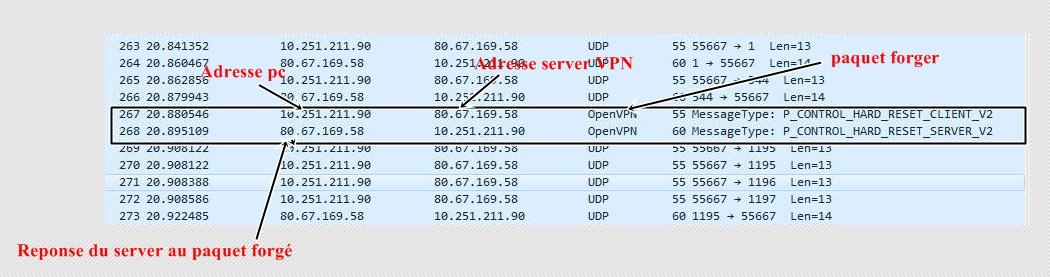
\includegraphics
[width=17cm]{scanudp.png}
\begin{center}
{\textbf{FIGURE 12:} SCAN TCP}
\end{center}
\begin{itemize}
\item[•] Utiliser les paquets UDP forgés pour scanner les ports du serveur en UDP, ceci ce fait en les envoyant au serveur en utilisant les sockets. Et Si on reçoit une réponse de la part du serveur VPN cela veut dire que le port via lequel le paquet UDP a était envoyer est ouvert.
\end{itemize}


%\subsubsection{diagrammes de séquence scan UDP}
\subsection {Amélioration du Scan des ports UDP/TCP}
Tout d’abord faut savoir que le server vpn-rw.fdn.fr écoute sur tous les ports (tous ces ports sont ouverts en TCP/UDP). Dans ce cas ce qui pourrait poser problème pour lancer une connexion avec le server VPN c’est le réseau sur lequel on est connecté (le fournisseur internet) car généralement les fournisseurs internet et administrateurs réseaux fermes certains ports pour des raisons de sécurité ou autre par exemple pour interdire l’utilisation des Torrent.\\

Mais avant de parler des modifications que nous avons apportées sur les Scans TCP/UDP par rapport à ceux implémentés auparavant, on explique d’abord pourquoi nous avons effectué ces changements.\\

Nous avons remarqué que lorsqu’on lançait plusieurs connexions en même temps sur le server VPN vpn-rw.fdn.fr sans lui fournir un login et un mot de passe valable, le server OpenVpn note le message d’erreur dans un coin et après un certain moment fail2ban finit par blacklister l’origine des connexions qui ont causé l’erreurs. (C’est notre client qui nous a donné ses remarques et informations car c’est l’une des personnes à gérer le server vpn de fdn).  Notons que ce comportement est propre au server vpn-rw.fdn.fr et que ça pourrai varier d’un server vpn a un autre.\\

De plus lorsque on reçoit une réponse que ça soit suite à un Scan Tcp ou un scan UDP on n’est pas sûr d’avoir reçu la réponse du server VPN il se pourrait que ça soit un proxy transparent.\\

Neutral-echo.aquilenet.fr: est un serveur "echo" mis en place par aquilenet (Fournisseur d'accès Internet libre en Aquitaine) ou tous les ports sont ouverts, et font tourner un simple cat, il suffit donc de s'y connecter avec telnet ou en TCP Ou UDP et d'essayer de taper quelque chose pour vérifier que le port passe bien. \\

Afin d’améliorer nos scan déjà implémenté nous avons utilisé le server neutral-echo.aquilenet.fr qui a la même caractéristique que le server vpn-rw.fdn.fr  ou il accepte les connexions sur tous les ports que ça soit en TCP ou en UDP et en plus sans demander de login Et lorsqu’il reçoit un paquet il renvoie tout simplement tout ce qu’on lui a envoyé. \\
\subsubsection{Scan TCP en utilisant aquilenet}
Le TcpScanWithAquilonet ()  et similaire au TcScan () ou on envoie une demande de connexion au server de aquilante on attends une réponse de la part du server , une fois la réponse reçu on envoie un paquet TCP A contenant une donnée  Data et on attends la réponse du server aquilenet  si la donner reçu dans le paquet de réponse et identique à la donnée Data envoyé cela voudrai dire qu’on a bien reçu la réponse de la part du server aquilenet et que le port via lequel nous avons envoyé le paquet A est ouvert .\\

Et si on ne reçoit pas une donnée identique à Data cela voudrait dire que nous n’avons pas reçu la réponse de la part du server aquilenet  et qu’il y a un proxy transparent qui tourne sur le port via laquelle nous avons envoyé le paquet A*.\\
\subsubsection{Scan UDP en utilisant aquilenet}
Le scan PortScanUdpWithAquilonet () consiste à envoyer le paquet UDP que nous avons déjà forgé au server aquilenet et si on reçoit une réponse de la part du serveur on vérifie si la data est exactement la même que celle qu’on a envoyé si c’est le cas cela voudrai dire que le port via lequel on a envoyé le paquet est ouvert et que le  paquet reçu vient bien du server aquilenet et que ce n’est pas une réponse de proxy qui tourne sur le port via lequel nous avons envoyé le paquet.\\
\subsection{Gestion de scan des ports }
Scanner les ports d’une manière basique qui est de commencer par le port 1 et de finir par le port 65 536 ce n’est pas la bonne approche car on pourra tomber sur des plages de ports qui sont fermés et on passera un moment à les scanner sans que cela ne donne de résultat.\\
Dans un souci d’amélioration de performance du scan des ports UDP/TCP nous avons devisé l’action scan port sur 3 Phases : \\
\begin{itemize}
\item[•] \textbf{phase 1 :} 
Elle  consiste à scanner les ports de la liste du niveau 1 en UDP puis en TCP, la liste de port du niveau 1 contient les ports les plus connus.  Si on ne trouve pas de port ouverts on passe à l’étape 2.\\
\item[•] \textbf{Phase 2 : }
Consiste à faire le scan des ports de la liste du niveau 2 en UDP puis en TCP, la liste de port du niveau 2 contient  ports qui  ne sont pas connu mais ils ont déjà trouvé comme port ouvert dans d’ancienne exécution de la phase 3 dès qu’un port ouvert est détecter on arrête le scan et en passe à la génération du fichier de configuration . Si cette phase-là ne détecte pas de ports ouverts on passe à la 3ème phase.\\ 
\item[•] \textbf{Phase 3 :}
Si aucun port ouvert n’est trouvé dans les deux phases de scan précédent on fait un scanne de port en UDP puis en TCP sur les 65 536 ports.\\

\subsubsection{PortScanManager ():}


La fonction PortScanManager () c’est la fonction qui fait la gestion du scan de port UDP/TCP avec les trois niveaux, en premier lieu on lance le scan des ports UDP (PortScanUdpWithAquilonet) sur liste du niveau 1 en parallèle, si un thread détecte un port ouvert les autres threads qui sont déjà lancés termine leurs exécutions et on passe à la génération de fichier de configuration.\\

Si on ne trouve aucun port ouvert en UDP on lance des scans de ports  TCP (TcpScanWithAquilonet) en parallèle en sur la liste du premier niveau si on trouve un port ouvert, les threads s’arrête et on passe à la génération du fichier de configuration. Sinon on passe au Scan des ports de la liste niveau 2.\\

Le même processus est répété pour le scan de ports de la liste Niveau2 sauf qu’avant de scanner les ports, on charge la liste de port niveau 2 à partir d’un fichier.txt ou on avait gardé les ports trouvé éventuellement lors des scans de port de la liste niveau 3.\\

Dans le scan des ports de la liste Niveau 3 qui contient l’intégralité des ports le  même processus est répété que dans le scanne niveau 1, la différence est que lorsque on trouve un port ouvert on l’enregistre dans le fichier contenant la liste des ports de niveau 2. \\
\end{itemize}
\subsection{Parallélisme des traitements}

Dans la partie de Thread, on scan plusieurs port en même temps,pour essayer  d'ugementer il vitesse de trouver le bon port. nous avons défini le nombre de thread \textbf{NumberThread = 20},car nous avons testé avec plus de 100 threads après le premier scan le site nous ajoute dans le black list et il nous considère comme une attaque méchante, du coup nous avons diminué le nombre de thread pour essayer d'avoir un nombre raisonnable.
\subsection{Interface}

Notre interface se compose de trois fenêtres qui sont:\\
\textbf{Fenêtre principale: }\\
\begin{center}
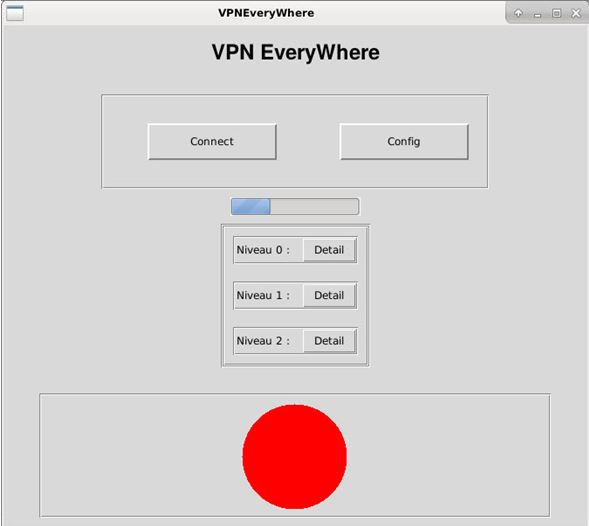
\includegraphics
[width=11cm]{VPNEveryWhere.jpg}
\end{center}
\begin{center}
{\textbf{FIGURE 13:} Fenêtre principale }
\end{center}


\begin{itemize}
\item Bouton Connect: permet le lancement de la connexion du client OpenVPN avec le serveur OpenVPN en passant par les étapes de scan de port en appelant la bibliothèque et mettre à jour le fichier de configuration\\
\item Bouton Config: permet de configurer les login, password et de changer le serveur et le certificat et mettre à jours ces informations dans le fichier de configuration.\\

\item Barre de progression: pour afficher l’avancement de la  recherche  par nombres des ports testés et niveau de recherche.\\

Et un bouton détail devant chaque niveaux pour avoir des informations sur le scan.
\end{itemize}

Voyant: on a trois état avec trois couleurs différentes
\begin{itemize}
\item Rouge  : déconnecté du serveur.
\vspace{8pt}
\item Orange : connexion en cours.
\vspace{8pt}
\item Vert   : connecté au serveur.\\
\end{itemize}

\textbf{Fenêtre Config: \\}
\begin{center}

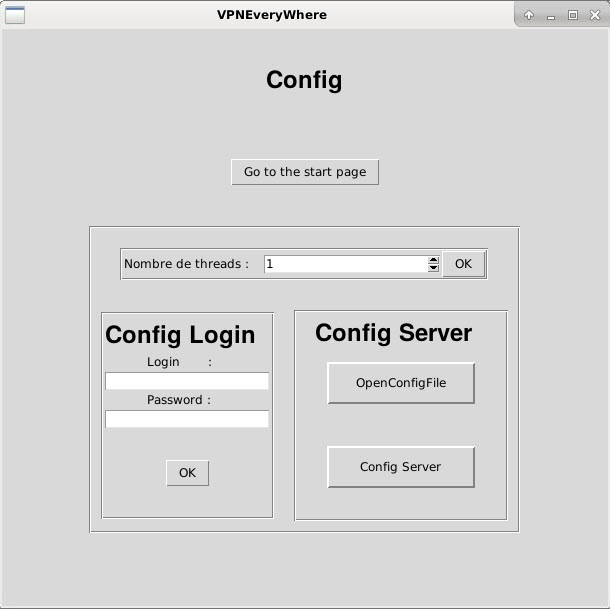
\includegraphics
[width=10cm]{Config.jpg}
\end{center}
\begin{center}

{\textbf{FIGURE 14:} Fenêtre Config}
\end{center}
\begin{itemize}
\item[] Selection du nombre de threads à lancer à la fois.

\item[] Changement du Login et password:
\begin{itemize}
\item[] Login: contient le nom d'utilisateur.\\
\item[] Password: pour le password de l'utilisateur.\\

En cliquant sur le bouton Ok le fichier de configuration sera modifié en mettant le nouveau Login ainsi que le nouveau password.\\
\end{itemize}
\item[] On cliquant sur le bouton ConfigServer on lance la fenêtre Server.

\end{itemize}
\textbf{Fenêtre Server \\}
\begin{center}
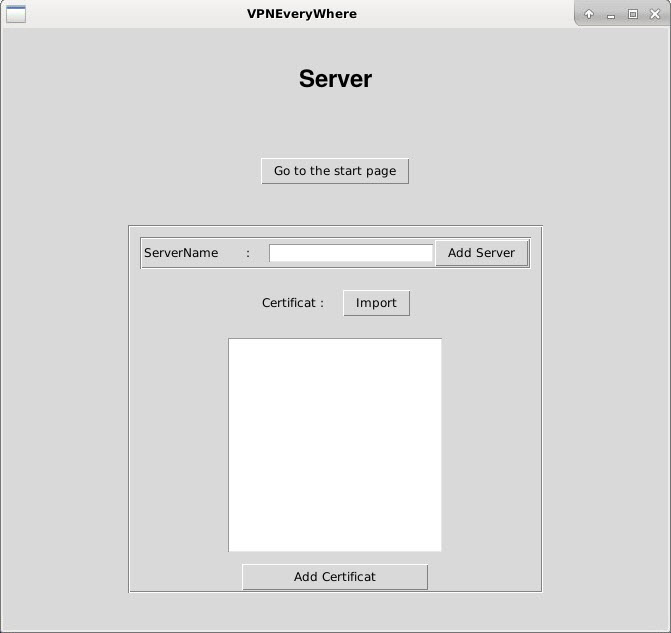
\includegraphics
[width=11cm]{Server.jpg}
\end{center}
\begin{center}
{\textbf{FIGURE 15:} Server }
\end{center}
\begin{itemize}

\item[] Server: pour configurer le serveur.\\

En cliquant sur le bouton Add Server, le fichier de configuration sera à jour en modifiant le serveur dans le fichier de configuration.


\item[] Certificat: pour changer le certificat.\\

Pour modifier le certificat et le mettre à jour dans le fichier de configuration, on a deux méthodes, soit en important le certificat à partir d'un fichier text soit faire du copier coller dans la zone de text.
\end{itemize}
\newpage

\subsection{Fichier de configuration}
Le fichier de configuration fournir par OpenVpn de FDN est utilisé pour imposer certains réglages, comme le protocole a utilisé, le Certificat qui permet de vérifier que c'est bien à FDN que l'on se connecte.

Après avoir finir le scan et trouver un port ouvert, une mise à jour automatique du fichier de configuration sera faite, en ajoutant le numéro de port et le protocole utilisé afin que le client puisse se connecter avec le serveur OpenVPN.

Notant que y a aussi la possibilité de configurer manuellement un serveur VPN, modifier le certificat utilisé ainsi que le login et password utilisé lors de l'autentification, afin de réussir la connexion avec le serveur.
\subsection{Lancement de serveur}
Quand le programme a trouvé le port ouvert et il lance automatiquement le client openvpn que l'utilisateur déjà installer sur son l'ordinateur et communiquer avec le serveur openvpn avec le ficher de configuration qu'on a générer.
\newpage

%\section{bibliothèque}
%La pratie de la bibliothèque a part, permet d'utiliser dans les autres project.\\


\newpage
\section{Tests}

D'abord, on ferme tout les ports, et on laisse seulement un port ouvert (par exemple 53), pour effectuer ce test, on tape les lignes de commande suivantes:\\
\begin{lstlisting}[keywordstyle=\color{blue!70}, commentstyle=\color{red!50!green!50!blue!50}, frame=shadowbox, rulesepcolor=\color{red!20!green!20!blue!20}]
iptables -A INPUT -p tcp --dport 53 -j ACCEPT
iptables -A OUTPUT -p tcp --dport 53 -j ACCEPT
\end{lstlisting}
Et puis on ferme tout les autres ports avec la commande suivante:\\
\begin{lstlisting}[keywordstyle=\color{blue!70}, commentstyle=\color{red!50!green!50!blue!50}, frame=shadowbox,
rulesepcolor=\color{red!20!green!20!blue!20}]
iptables -P OUTPUT DROP
iptables -L -n /*pour verifier si le port sont DROP */
\end{lstlisting}

On lance notre programme pour essayer le scan des ports, et on doit trouver le même port qu'on a laisser comme résultat de la bibliothèque de scan, cela signifie que notre scan donne des bons résultats.\\

\subsection{Tests unitaires}

Une des grandes préoccupations lors de développement des logiciels est d’être certains que l'application fonctionne et surtout quelle fonctionne dans toutes les situations possibles et qu'elle renvoie les résultats attendus.  

Pour tester notre application et ses différentes fonctionnalité nous avons implémenté des fonctions de tests unitaire sur les différentes parties.\\[0.5cm]


{\textbf{Test de Scan:}}

Le plus important est de tester le scan et de vérifier s'il renvoi bien les résultats attendu, pour ça on a le test suivant : 
\begin{center}
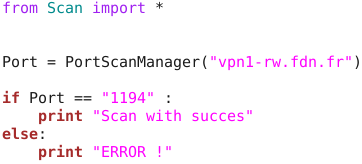
\includegraphics
[width=10cm]{Test_Scan.png}

{\textbf{FIGURE 16:} Test unitaire du Scan "PortScanManager()"}
\end{center}

Afin de tester si notre scan de port marche nous avons scanner Le serveur vpn1-rw.fdn.fr écoute uniquement sur le port 1194, et le test vérifier bien si la fonction retourne le bon port.

{\textbf{Test du changement de certificat}}\\
\begin{center}
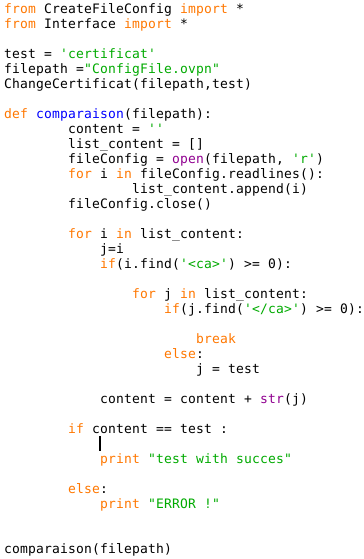
\includegraphics
[width=7cm]{test_changeCertificat.png}

{\textbf{FIGURE 17:} Test unitaire du changement de certificat"}
\end{center}

Ce test est basé sur la comparaison du certificat du fichier de configuration après la modification avec celui que l'utilisateur vient de mettre dans l'interface.

\subsection{Tests de fonctionnement de la bibliothèque Scan}

Un petit script python a été mis en place afin de vérifier que la bibliothèque ne dépend pas des autres classes, en faisant appel à PortScanManager et lui donner l'adresse du serveur en paramètre, le scan se lance.\\
\begin{center}
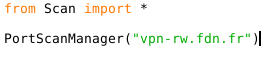
\includegraphics
[width=5cm]{TestBiblio.png}
{\Huge $\rightarrow$}
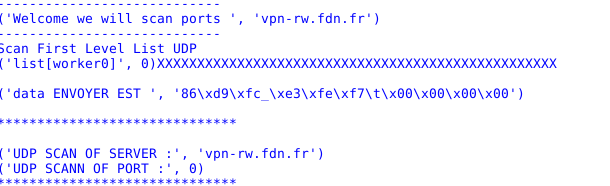
\includegraphics[width=8cm]{TestBiblio2.png}\\
{\textbf{FIGURE 18:} Test de la bibliothèque}
\end{center}

On a testé la bibliothèque de scan sur le serveur 80.67.169.57 qui écoute seulement sur le port 1194, et voici le résultat de ce test:
\begin{center}
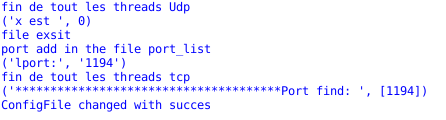
\includegraphics
[width=10cm]{Test1.png}
\end{center}
\begin{center}
{\textbf{FIGURE 19:} Test bibliothèque}
\end{center}

On voit sur la figure, que la bibliothèque de scan retourne comme résultat le port 1194 qui est le seul port ouvert sur le serveur 80.67.169.57 ce qui montre que le scan fonctionne bien et arrive à trouver le bon port.

\subsection{Tests de fichier configuration}
Après avoir finir la mise à jour du fichier de configuration, le fait de pouvoir se connecter au serveur OpenVPN avec le fichier qu'on a adapté signifie que ce dernier a pris en compte la bonne configuration(port, proto, certificat ...).

\subsection{Tests de fonctionnement}
\subsubsection{Tests du bon fonctionnement de la bibliothèque de scan}
\textbf{Type de test: Test de fiabilité}\\
\textbf{Objectif: } comparaison des résultats de notre bibliothèque et celles de la bibliothèque nmap.\\
\textbf{Raison de ce test: }Nmap (“Network Mapper”) est un outil qui fonctionne très bien et fiable pour le scan des ports et qui donne des bons résultats.

Au début, on voulais effectuer notre test de port à l'aide de la bibliothèque Nmap, mais puisque cette dernière ne donne pas de résultats pour le scan UDP, on l'a fait autrement et dans ce qui suit le diagramme de séquence du scan nmap:\\

\textbf{Réalisation de test:}\\

On lance notre application pour scanner tous les ports dès qu'on trouve un port ouvert on l'ajoute dans un fichier 2, et puis on lance le scan avec la biblioteque Nmap et on fait la même chose, si on trouve un port on ajoute dans le fichier 1.\\

Après avoir les deux fichers, on lance le programme \textbf{comparer\_port} pour comparer les ports dans les deux ficher pour voir le taux de différence entre les deux fichier.\\
voici les figures de résultat obtenu:
\begin{center}
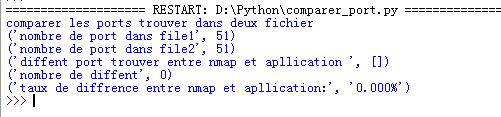
\includegraphics
[width=10cm]{comparerport1.png}
\end{center}
\begin{center}
{\textbf{FIGURE 20:} Comparaison des ports niveau 1}
\end{center}
\begin{center}

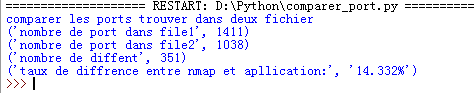
\includegraphics
[width=10cm]{comparerport2.png}
\end{center}
\begin{center}
{\textbf{FIGURE 21:} Comparaison des ports niveau 3}
\end{center}
On peux voir dans la partie niveaux 3, que y a  une différence entre le scan nmap et l'application, la raison est que dans notre bibliothèque de scan, on attend la réponse du serveur dans un temps limité et s'il répond pas rapidement on avance le scan des autres ports pour gagner du temps. \\

Une autre raison est que notre bibliothèque de scan fait la différence entre un proxy transparent et un vrai serveur (ce qui est expliqué dans la partie scan), qu'on lui envoie un message et s'il répond par le même paquet qu'on a envoyé, cela veut dire que c'est un vrai serveur et pas un proxy. mais du coté de nmap il dit que le port est ouvert s'il lui répond et sans même pas vérifier le contenue du paquet reçu. Du coup on trouve moins de port ouvert par rapport ce lui de nmap et c'est ce qui est logique. 
%\subsection{Remarque}
\newpage
\section{Conclusion}
\begin{flushleft}
\Large\textbf{Bilan }
\end{flushleft}

Ce projet nous a permis de nous initier au domaine des VPNs, il nous a aussi permis d'avoir nouvelles compétences en réseaux informatique. 

Nous avons terminé le travail demandé par le client, tous les besoins fonctionnels ont été réalisés,la   bibliothèque de Scan de ports UDP/TCP en python , la mise à jour du fichier de configuration avec le port ouvert trouvé et éventuellement Login, password du client,la possibilité de configurer un server VPN manuellement en ajoutant son certificat  son nom de domaine etc ... , et nous avons réaliser le lancement automatique de connexion avec le serveur VPN de FDN qui etait le denier besoin fonctionnel a réaliser .\\
\begin{flushleft}
%\Large\textbf{Perspectives }
\end{flushleft}
\newpage

\section{Bibliographique}
\bibliographystyle{alpha}
%\begin{itemize}
%\item Le livre \cite{Chr02} pour apprendre le programme python.
%\item Le website \cite{Fou16} 
%\item Le website \cite{Lyo16} qui parle de la biblioteque nmap
%\end{itemize}
\nocite{*}
\bibliography{bibliographique}

\end{document}


